\documentclass[a4paper,12pt]{article}

\usepackage{graphicx}
\usepackage{hyperref}
\usepackage{amssymb}
\usepackage{amsmath}
\usepackage{listings}
\usepackage{pgfplots}
\usepackage{breqn}

\pgfplotsset{compat=1.16}
\lstset{frame=tb,
  aboveskip=3mm,
  belowskip=3mm,
  columns=flexible,
  basicstyle={\small\ttfamily}
}

\title{Calculus --- Summary}
\author{Dany Sluijk}
\date{November 2018}

\makeindex

\begin{document}
\maketitle
\begin{center}
	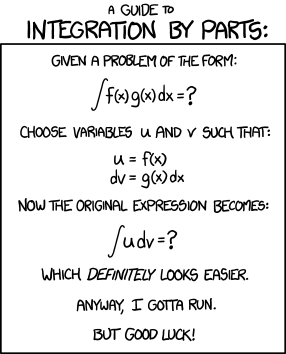
\includegraphics[height=9cm]{./intro}
\end{center}
\begin{abstract}
	This document contains a summary of the Calculus course given
	in the first year of Computer Science and Engineering.
	This is \emph{not} a definitive guide, and might contain errors.
	Please send an email to \href{mailto:dany@atlasdev.nl}{``dany@atlasdev.nl''}.
	This summary is distributed under the
	\href{https://opensource.org/licenses/MIT}{MIT} license.
\end{abstract}

\newpage
\tableofcontents

\section{Limits}
Limits are the foundation of calculus.
A lot of other things commonly used in calculus are made with the help of limits.
For example the derivative of \(x^2\) is \(2x\).
This can be proven by using limits.
A limit of a function is the value of the function when it approaches a value.

\subsection{Limit law}

Given two limits \(\lim_{x \to a} f(x)\) and \(\lim_{x \to a} g(x)\) we can say that:

\begin{table}[h]
	\centering
	\begin{tabular} {c}
    \(\lim_{x \to a} [f(x) + g(x)] = \lim_{x \to a} f(x) + \lim_{x \to a} g(x)\) \\\hline
    \(\lim_{x \to a} [f(x) - g(x)] = \lim_{x \to a} f(x) - \lim_{x \to a} g(x)\) \\\hline
    \(\lim_{x \to a} [c f(x)] = c \lim_{x \to a} f(x)\) \\\hline
    \(\lim_{x \to a} [f(x)g(x)] = \lim_{x \to a} f(x) * \lim_{x \to a} g(x)\) \\\hline
    \(\lim_{x \to a} \frac{f(x)}{g(x)} = \frac{\lim_{x \to a} f(x)}{\lim_{x \to a} g(x)} \text{if} \lim_{x \to a} g(x) \neq 0\) \\
	\end{tabular}
	\caption{Limit laws}
\end{table}

\subsection{Finding a limit}
\begin{figure}[h]
  \begin{center}
    \begin{tikzpicture}
      \begin{axis}[
          axis x line=center,
          axis y line=center,
          xtick={-5,-3,...,5},
          ytick={0,0.5,...,2},
          xlabel=$x$,
          ylabel=$y$,
          xmin=-5,
          xmax=5,
          ymin=0,
          ymax=2,
          samples=5
        ]
        \addplot [color=blue] {(x-1)/(x-1)};
        \legend{\((x-1)/(x-1)\)}
      \end{axis}
    \end{tikzpicture}
  \end{center}
\end{figure}

The simplest way of approximating the limit,
is to evaluate the function with an \(x\) close to the limit you want.
Take for example the function graphed above.
\(f(1)\) is obviously not defined, you cannot solve it that way.
But you can approximate it by filling \(1.00000001\) into the function.
This gives \(1\), which is the limit.

\subsection{Doing it properly}
This does not always work, so it's better to rewrite the function.
For example:

\[
  f(x) =
  \frac{x-1}{x-1} =
  \frac{1}{1} =
  1
\]

Obviously this is a simple function, other functions will not be this simple.
For example, solving the following function will look like this:

\begin{dmath}
  \lim_{x \to 0} \frac{\sqrt{x^2 + 9} - 3}{x^2} =
  \lim_{x \to 0} \frac{\sqrt{x^2 + 9} - 3}{x^2} * \frac{\sqrt{x^2 + 9} + 3}{\sqrt{x^2 + 9} + 3} =
  \lim_{x \to 0} \frac{(x^2 + 9) - 9}{x^2(\sqrt{x^2 + 9} + 3)} =
  \lim_{x \to 0} \frac{1}{\sqrt{x^2 + 9} + 3} =
  \frac{1}{\sqrt{0^2 + 9} + 3} =
  \frac{1}{6}
\end{dmath}

\subsection{Continuity}
A function is {\bf continuous} iff

\begin{itemize}
  \item \(f(a)\) is defined
  \item \(\lim_{x \to a} f(x)\) exits
  \item \(\lim_{x \to a} f(x) = f(a)\)
\end{itemize}

So, \(f\) is continuous at \(a\) if \(f(x)\) approaches \(f(a)\).
If this is not the case we can say that te function is {\bf discontinuous at a}.

\subsection{Limits at infinity}
If you take an infinity positive or negative number as the limit you can get the horizontal asymptotes of a function.
Take for example the following function:

\begin{figure}[h]
  \begin{center}
    \begin{tikzpicture}
      \begin{axis}[
          axis x line=center,
          axis y line=center,
          xtick={-20,-10,...,20},
          ytick={-2,-1,...,2},
          xlabel=$x$,
          ylabel=$y$,
          xmin=-20,
          xmax=20,
          ymin=-2,
          ymax=2,
          samples=75
        ]
        \addplot [color=blue,domain=-20:20] {(x^2-1)/(x^2+1)};
        \legend{\((x^2-1)/(x^2+1)\)}
      \end{axis}
    \end{tikzpicture}
  \end{center}
\end{figure}

This function probably has a horizontal limit at \(y=1\).
But you don't know for sure.
You can use the limit of infinity to prove them.
As constants don't really matter when approaching infinity you can remove them.
So you'll get the following:

\[
  \lim_{x \to \infty} \frac{x^2-1}{x^2+1} =
  \frac{\infty^2-1}{\infty^2+1} =
  \frac{\infty^2}{\infty^2} =
  \frac{1}{1} =
  1
\]

This gets the horizontal asymptote on the right.
If you want to get the limit on the left you'll have to use negative infinity.

\[
  \lim_{x \to -\infty} \frac{x^2-1}{x^2+1} =
  \frac{-\infty^2-1}{-\infty^2+1} =
  \frac{-\infty^2}{-\infty^2} =
  \frac{1}{1} =
  1
\]

In this example it's also \(y=1\), as both asymptotes are the same.
One important thing to keep in mind when solving infinite limits is that \(\frac{1}{\infty} = 0\).

\end{document}